\begin{frame}
\frametitle{Catmullrom}
  \begin{figure}[h]
  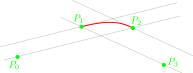
\includegraphics[width=5cm,keepaspectratio]{pics/catmullrom/catmullrom}
  \end{figure}
  {\scriptsize
    $$
v(t)=(1,t^1,t^2,t^3)\cdot
\frac{1}{2}\cdot
\left(
\begin{array}{cccc}
 0 &  2 &  0 &  0 \\
-1 &  0 &  1 &  0 \\
 2 & -5 &  4 & -1 \\
-1 &  3 & -3 &  1
\end{array}
\right)
\cdot
\left(
\begin{array}{c}
  {\color{green}P_{0}} \\
  {\color{green}P_{1}} \\
  {\color{green}P_{2}} \\
  {\color{green}P_{3}} 
\end{array}
\right)
$$
  }
\end{frame}

\begin{frame}
\frametitle{Catmullrom}
  \begin{figure}[h]
  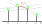
\includegraphics[width=5cm,keepaspectratio]{pics/catmullrom/catmullrom2}
  \end{figure}
  {\scriptsize
    \[
    \begin{array}{ccc}
      f(0) &=& {\color{green}P_1} \\
      f(1) &=& {\color{green}P_2} \\
     f'(0) &=& \frac{{\color{green}P_2}-{\color{green}P_0}}{2} \\
     f'(1) &=& \frac{{\color{green}P_3}-{\color{green}P_1}}{2} \\
      f(t) &=& \sum\limits_{i=0}^{i \leq 3}(a_i+b_it+c_it^2+d_it^3){\color{green}P_i}
    \end{array}
    \]
  }
\end{frame}

